\documentclass{article}%
\usepackage[T1]{fontenc}%
\usepackage[utf8]{inputenc}%
\usepackage{lmodern}%
\usepackage{textcomp}%
\usepackage{lastpage}%
\usepackage[head=40pt,margin=0.5in,bottom=0.6in]{geometry}%
\usepackage{graphicx}%
%
\title{\textbf{Tarek William Saab: Autopsia esclarece que Fernando Albán se suicidó}}%
\author{ANTONELLA DE VITA}%
\date{14/10/2018}%
%
\begin{document}%
\normalsize%
\maketitle%
\textbf{URL: }%
http://www.eluniversal.com/politica/23158/tarek{-}william{-}saab{-}autopsia{-}de{-}esclarece{-}que{-}se{-}suicido\newline%
%
\textbf{Periodico: }%
EU, %
ID: %
23158, %
Seccion: %
politica\newline%
%
\textbf{Palabras Claves: }%
NO\_TIENE\newline%
%
\textbf{Derecho: }%
1.1, %
Otros Derechos: %
1.10, %
Sub Derechos: %
1.1.1.3, 1.10.1\newline%
%
\textbf{EP: }%
NO\newline%
\newline%
%
\textbf{\textit{El fiscal general de la República designado por la Asamblea Nacional Constituyente aseguró que Albán "iba a ser presentado por su vinculación con el atentado. En su teléfono se encontraron pruebas”}}%
\newline%
\newline%
%
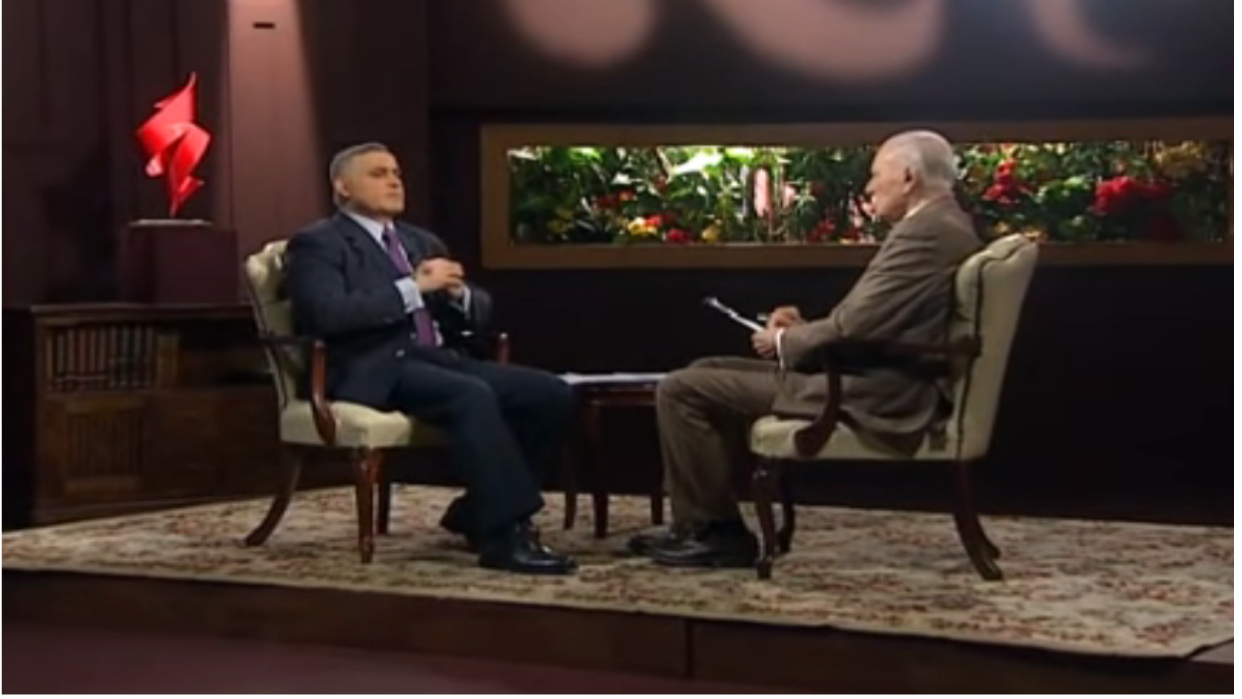
\includegraphics[width=300px]{153.jpg}%
\newline%
%
Durante una entrevista en el programa dominical José Vicente Hoy, que transmite Televen, Saab aseveró que “los resultados de la autopsia de Fernando Albán, esclarecen que el ciudadano se suicidó”. Es la respuesta del fiscal ante la exigencia de la comunidad internacional de solicitar una investigación independiente.“Burlando su propia condición de privado de libertad, se encontraba en la oficina administrativa, pidió ir al baño, y allí decidió lanzarse por la ventana y allí la autopsia es clave, auditable para quien  quiera. Él cae, incluso, con signos vitales” (…) "Iba a ser presentado por su vinculación con el atentado. En su teléfono se encontraron pruebas”, señaló.Asimismo, Saab declaró que “él muere por un choque hemorrágico. Es obvio que al lanzarse de un décimo piso no tenga ese desenlace fatal. Entonces está la autopsia, están las fotografías, están las entrevistas que hemos hecho a quienes en ese momento se encontraban con él”.%
\newline%
%
\end{document}